\subsection{Development process, methodology and work flow}

We started on this project as part of a course work for TDT4290 Customer
Driven Project. In this project, we have been able to walk through the processes
of software development efforts an average software engineer would have gone
through in an industrial setting. We have also tried to use our own experiences
and practices to improve upon industry accepted standards. 
This gave us an invaluable insight into how we handle, schedule,
manage, trace and carry out tasks in software development projects and below is
an evaluation of our experience in this project.

	\subsubsection{Development methodology---Scrum}

With scrum being the most popular software development methodology these days
plus the fact that all the team members had some sort of experience with it
helped save a considerable amount of time we would have spent learning the
basics of scrum. However, adopting pure scrum  was not reasonable since all team
members had responsibilities in other courses with demanding projects, and
attending five days of stand up meeting consistently by all group members was
unrealistic. Scrum is also complex administrative wise and we felt that adopting
pure scrum would take focus away from the actual project. 

To make sure such things went smoothly, we had to get together early and decide
on what methodology to use, or alternatively, what parts we would like to
employ from a given methodology. 

We decided to hold a stand-up meeting, a time slot when everyone will
be able to inform other members of self-completed task and plan for the day
ahead, to keep everyone up to speed with the project progress. We also fixed
sprint lengths to maximum of two weeks. We found this to be very effective in
terms of motivation and progress for the project. We borrowed the term product
owner and scrum master from the SCRUM methodology, and negotiated with the
customer to have just one person making the calls about the project.

One of the most challenging things to do was to wake up early and show up every
Monday to Thursday morning at 9 to work. Some group members work late
into the night and making it early in the morning was a bit of an inconvenience.
However, we decided to stick to the plan and that has helped us complete a greater
portion of requirements gathering and analysis task early for approval with our
customer. 

We did not use a SCRUM board for our project. Instead we depended on oral 
communication and work tasks for a given day was given at each standup meeting.
At times, we had to explicitly assign tasks if we felt that some
unpopular tasks were being bounced around. These were often given a deadline for
completion, and each team member committed to completing their work tasks they
set for themselves each day.

In general, the flexible division of work and the consistent stand-up meeting
worked out great, and we did not feel that the methodology took time from actual
development and documentation. 

	\subsubsection{Implementation}
The implementation would have been simpler and perhaps faster had it been an
application that was going to be deployed on either Android or iOS platforms as
native application.

But the requirement was that the application should have one code base and run
on both platforms.
It is a cross-platform application.
None of us had any experience with that sort of thing, so the natural thing to
do was to make sure every one of us evaluated some framework for the
implementation of the requirement.
A number of frameworks came on the table and we had to weigh one against another.
We selected the relatively new PhoneGap for many reasons, as specified in detail
in earlier sections of this project document.
Learning the new framework, getting to know existing API's from our customer and
on how we were going to integrate our solutions to the customer requirements
provided its own challenges.
And we also wanted to develop an application that not only did the
functionalities but also have some elegant interface which is less confusing and
appealing to end users.

The use of PhoneGap in collaboration with JQuery Mobile made the design of our
UI very simple and gave us additional time for shaping the application itself.
Our customer also provided us with a style-sheet used in their online touch
device portal so that the designs would match.  Although being a great framework
for our purpose, PhoneGap also had it's shortcoming.  Because it's a
script-language run in the web-application of the mobile device it's performance
is limited compared to a standalone native app.  This downside is also
observable in our app, the responsiveness and page transitions are noticeably
slower than what would've been the case for a native app.  However we believe
this is within reasonable limits and further improvements could possibly make it
faster.

The implementation took place in line with our requirements elicitation, working
first on the highest priority and starting early on high complexity
requirements.  The implementation needed a collaboration between the group
members who were investing so much effort on the codes and we used GitHub for
listing issues and tracing changes.

In general, we had exactly 10 requirements of which four were high priority and
one with high complexity.  Nine of the ten requirements were successfully
implemented according to the customer's requirements.  The final requirement was
quite complex and also goes against mobile app conventions so it wasn't feasible
to implement within our scheduled time. (TODO refer to where this is discussed)

	\subsubsection{Time estimation}
  This project lasted from week 35 until week 47. During this time, we decided
  the work into three blocks of time. Pre-study, implementation and
  documentation. 
  
  For the first three weeks, we spent most of our time doing
  requirements gathering, background study of the problem domain and decided
  methodologies and technologies to be used for the project.

  The next eight weeks, we did 4 sprints of two weeks each. For each sprint we
  created a sprint backlog, completed it and documented our efforts. We had
  planned for 350 person hours for each sprint, but we found that we used less
  time than that completing our sprints. 

  For the final two weeks we reflected on our work, wrote the discussion and
  evaluation chapter, and worked on how the project could be improved from here.
  We alloted 350 person hours for this reflection, and found that we needed most
  of it to completely reflect and document our efforts. 
  
  \paragraph{Day to day workflow}
  Our usual workflow started with a standup every morning at 09.15 at Drivhuset.
  We spent about 15 minutes discussing the previous day, and the tasks ahead of
  us. After this, we sat together and worked most of the time, and let the group
  members that needed to attend other lectures go when needed. Each group member
  committed to completing his work tasks set by the stand up meeting that day,
  but how and when he did it, was up to each group member himself. On average,
  each day consisted of 6 hours of work, with Fridays off. We found this method
  of working very efficient, and no one felt overworked or demotivated because
  of it.

  \paragraph{Seminars and meetings}
  In addition to the project, we also had to attend seminars and meetings. Every
  Tuesday at 14.00, we had seminars in group dynamics and project management.
  These seminars took an average of 2 hours each week during the project. 

  We also had a mandatory advisor meeting at 13.00 every Tuesday. This proved
  invaluable to the project success, and our advisor helped us greatly. 
 	
    \begin{figure}[htb]
        \centering
        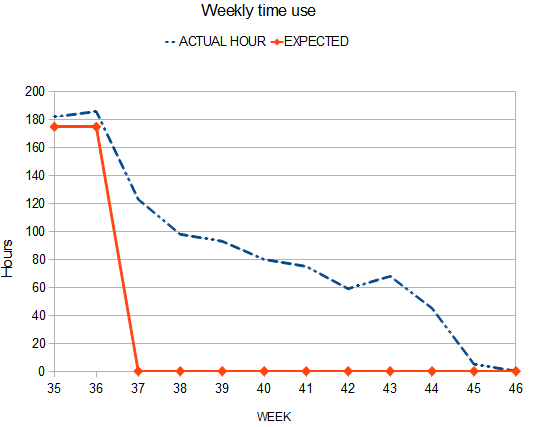
\includegraphics[scale=0.88]{timebudget.png}
        \label{fig:time}
    \end{figure}
	
	\subsubsection{Seminars and study process}
  The group attended a lot of seminars organized by IDI for this course. Some of
  the most important seminars were:
	
  \subparagraph{Group dynamics} - one of the first and maybe most important
  seminar showed values of good team work and importance of correct
  communication inside the team. It helped people in group to understand mutual
  differences and to achieve better communication without knowing other persons
  before. Also, it was nicely explained how team work should lead to better
  efficiency and more productivity, and it is always good to hear something
  about that from experienced people working with big groups for a long time.

  \subparagraph{Project management} - this seminar revolved around efficient
  management of big project like this one. We learned about how a project should
  be defined, how to find the goal objectives, and starting points for the
  development process. 
  
   \subparagraph{Scrum, an agile development method} - Considering scrum as one
   of the most used method for developing software in past years, everyone had
   basic knowledge about it.  The group felt that this seminar came little late
   for any major change in our plan.  

  \subparagraph{Technical writing} - This seminar, held by prof. nancy Lea
  Eik-Ness thought us about the flow of articles and documents for this project.
  This lecture was held after our preliminary delivery, and proved valuable for
  the quality of our final report. In addition to this, we also got valuable
  feedback on our own report.

  \subparagraph{Presentation techniques} - This seminar focused on presentation
  technique, which proved valuable to the project before the final presentation
  of the project.

  These seminars were invaluable to the success of our project. It motivated us,
  and gave us important insight into the group dynamics and goals of the
  project.

